\chapter{Transformers}
\begin{note}{Reference}
    Chris and Hugh Bishop, Deep Learning: Foundations and Concepts \cite{bishop2023deep}.
    Chapter 12.
\end{note}

A transformer is a model that transforms a set of vectors into another set of vectors in a space of the same dimensionality. The goal of the transformation is to obtain vectors with a better internal representation for solving the task, e.g., to give the correct interpretation to the words in a sentence.

\section{Attention}
Consider the following sentences:
\begin{itemize}
    \item \textit{I swam across the river to get to the other bank.}
    \item \textit{I walked across the road to get cash from the bank.}
\end{itemize}

According to the distributional hypothesis, to give the correct interpretation to the word \textit{bank}, it is necessary to analyze its context. 
In particular, to give the correct interpretation to \textit{bank}, one must pay greater \keyword{attention} to the words \textit{swam} and \textit{river} (in the first sentence) and \textit{cash} (in the second sentence).

Note that attention should not be based solely on the position of a word in a sentence. Indeed, the words \textit{swam}, \textit{river}, and \textit{cash} might appear in different positions for different inputs, but this does not mean they should be given less attention. 
As we noted in the previous chapter, this desired property contrasts with traditional neural networks, where the input $x_i$ is always multiplied by the same weight $w_i$. 
RNNs solve this problem, but here in this chapter we are proposing another, more efficient architecture.

\section{Computation}
The input to a transformer is a set of $N$ embedding vectors $\{\mathbf{x}_i\}$, each with $D$ dimensions. 
Each vector is a \textbf{token}.
The individual components $\mathbf{x}_{ij}$ of a token are called \textbf{features}.

Tokens are represented by an embedding matrix $\mathbf{X}$ of size $N \times D$, where the $i$-th row corresponds to the token $\mathbf{x}_{i}$.

We want to transform the input tokens $\mathbf{x}_{1:N}$ into output tokens $\mathbf{y}_{1:N}$ such that the latter have a better representation for solving the problem. The value of a single $\mathbf{y}_i$ must depend not only on $\mathbf{x}_i$ but on all tokens $\mathbf{x}_{1:N}$, and in particular on those tokens $\mathbf{x}_{k}$ that are especially important for determining the meaning of $\mathbf{y}_i$.

A simple way to achieve this is to consider each $\mathbf{y}_i$ as a linear combination of the tokens $\mathbf{x}_{1:N}$:
\[
\mathbf{y}_{i}=\sum^{N}_{j=1}a_{ij}\mathbf{x}_{j}
\]
where the $a_{ij}$ are called \keyword{attention weights}. An attention weight $a_{ij}$ should have a low value if $\mathbf{x}_{j}$ is irrelevant to the interpretation of $\mathbf{y}_i$, and a high value if it is highly relevant.

We want attention to be non-negative and for the sum of attention weights to be 1, so that paying more attention to one token means paying less to others.
Under these assumptions, if $a_{ij} = 1$, then $\mathbf{x}_j = \mathbf{y}_i$.

\section{Self-attention}
In the previous chapter, we introduce the attention concept for the first time. 
We said that it is a trainable mechanism to dynamically give attention to tokens of sequence \(\mathbf{x}_{1:N}\) for the output of the downstream task.
Now, consider the output being a sequence of tokens \(\mathbf{y}_{1:N}\). In this setting, the attention mechanism is creating a link between each of the input tokens and each of the output tokens.
We call \keyword{self-attention} the attention mechanism between the input sequence \(\mathbf{x}_{1:N}\) and itself, that is each input token has an attention coefficient for each on the other input tokens.
This mechanism allows to find out the most important tokens to attention when looking at each token \(\mathbf{x}_i\) of the sequence.

\begin{note}{An information retrieval metaphor}
    Suppose a user is searching for a movie to watch on an online platform, and the platform's search is implemented using a multimedia database where each movie (\textit{value}) has a set of attributes summarized in a key (\textit{key}). The user enters their desired attributes, which are summarized into a \textit{query} of the same type as the \textit{keys}. At this point, the database performs a similarity comparison between the \textit{keys} and the \textit{query} and returns one or more movies (\textit{values}).

    If the search engine returns a single \textit{value}, this is called \textbf{hard attention}, as the user pays a lot of attention to that single \textit{value}. If, instead, the engine returns multiple \textit{values}, this is called \textbf{soft attention}, as the user distributes their attention among the returned \textit{values}. If the individual attention levels are continuous, differentiable, and trainable variables, then gradient descent can be used.

    We can view the token $\mathbf{x}_{i}$ as a \textit{value} and as its own \textit{key}. Then, we use the token $\mathbf{x}_{j}$ as a \textit{query} for the output token $\mathbf{y}_{j}$. In this way, to determine $\mathbf{y}_{j}$, we must compute the similarity between each token and $\mathbf{x}_{j}$, and thus the level of attention that $\mathbf{x}_{j}$ should pay to each of the tokens.

    This process is called \textbf{self-attention} because the same sequence is used to determine the \textit{queries}, \textit{keys}, and \textit{values}.
\end{note}

An attention coefficient $a_{ij}$ must measure how much attention should be paid to $\mathbf{x}_j$ to determine the meaning of $\mathbf{x}_{i}$. 
One way to measure this is by evaluating their similarity. 
The dot product is often used for this purpose and is a more computationally reasonable choice than the Euclidean distance. 
However, $\mathbf{x}_i^T \mathbf{x}_{j}$ could be negative and greater than 1. 
To satisfy the previously introduced constraints, we apply the $\text{Softmax}$ function to it:
\[
a_{ij}=\frac{\exp(\mathbf{x}_i^{T}\mathbf{x}_{j})}{\sum_{j'=1}^{N}\exp (\mathbf{x}_i^{T}\mathbf{x}_{j'})}
\]

The architecture described so far can be defined as:
\[
\begin{aligned}
\mathbf{Y} &= \mathbf{A}\mathbf{X}
\mathbf{A} &= \text{Softmax}\left[\mathbf{X}\mathbf{X}^{T}\right]
\end{aligned}
\]
where $\text{Softmax}\left[\mathbf{L}\right]$ is an operator that applies $\exp$ to each $l \in \mathbf{L}$ and normalizes each row to 1.

However, the coefficients obtained this way cannot be trained. Additionally, the features of individual tokens have the same weight, whereas it would be desirable to pay attention to specific features when computing the similarity between tokens.

We can solve both problems by assigning each vector $\mathbf{x}_i$ a trainable weight vector $\mathbf{u}_i$, so that each resulting vector is of the form $\mathbf{x}_{i}^{T}\mathbf{u}$. 
Considering all tokens involved, we assign a weight matrix $\mathbf{U} \in \mathbb{R}^{D \times D}$ to the token matrix $\mathbf{X} \in \mathbb{R}^{N \times D}$ s.t. \(\mathbf{X}\mathbf{U}\in \mathbb{R}^{N\times D}\).

Thus, the computation becomes:
\[
\begin{aligned}
\mathbf{Y}&=\mathbf{A}\left(\mathbf{X}\mathbf{U}\right)
\mathbf{A}&=\text{Softmax}\left[\mathbf{X}\mathbf{U}\mathbf{U}^{T}\mathbf{X}^{T}\right]
\end{aligned}
\]

However, the matrix $\mathbf{X}\mathbf{U}\mathbf{U}^{T}\mathbf{X}^{T}$ is symmetric, so the currently implemented attention mechanism is symmetric, whereas we want attention to be strongly asymmetric. For example, the attention that should be paid to the word \textit{hammer} to understand the word \textit{tool} is much greater than the reverse, since a \textit{hammer} is certainly a \textit{tool}, but a \textit{tool} is not necessarily a \textit{hammer}.

To introduce asymmetry, instead of using $\mathbf{U}$ as the weight matrix for \textit{query}, \textit{key}, and \textit{value}, we introduce three distinct weight matrices:
\[
\begin{aligned}
\mathbf{Q}&=\mathbf{X}\mathbf{W}^{(q)},\:\mathbf{W}^{(q)} \in \mathbb{R}^{D \times D_q} \\
\mathbf{K}&=\mathbf{X}\mathbf{W}^{(k)},\:\mathbf{W}^{(k)} \in \mathbb{R}^{D \times D_k} \\
\mathbf{V}&=\mathbf{X}\mathbf{W}^{(v)},\:\mathbf{W}^{(v)} \in \mathbb{R}^{D \times D_v}
\end{aligned}
\]

In this way, the computation becomes:
\[
\mathbf{Y}=\text{Softmax}\left[\mathbf{Q}\mathbf{K}^{T}\right]\mathbf{V}
\]

Given this structure, it is clear that $\mathbf{Q}$ and $\mathbf{K}$ must be compatible, as must $\mathbf{Q}\mathbf{K}^{T}$ and $\mathbf{V}$. To achieve this, it is necessary that $D_q = D_k$. Note also that it is $D_v$ that determines the size of $\mathbf{Y}$. Indeed, $\mathbf{Y} \in \mathbb{R}^{N \times D_v}$.

\begin{figure}[h]
    \centering
    \caption{A visualization of attention coefficients.}
    \label{fig:attention_coefficients}
    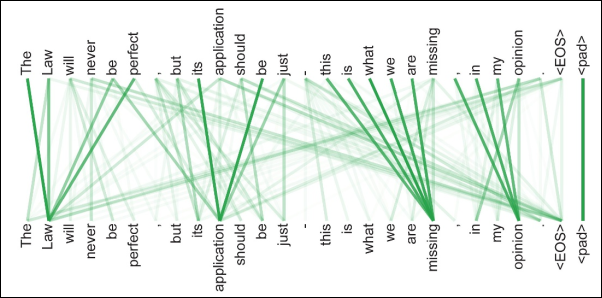
\includegraphics[width=0.6\textwidth]{_files/_images/attention_coefficients}
\end{figure}

Moreover, $\text{Softmax}$ has extremely small gradients for inputs with large absolute values. For this reason, we normalize the product $\mathbf{Q}\mathbf{K}^{T}$ by $\sqrt{D_k}$. This has a statistical foundation: if the components of the \textit{key} and \textit{query} vectors were i.i.d. as $\mathcal{N}(0,1)$, their dot product would have a variance of $D_k$ and thus a standard deviation of $\sqrt{D_k}$. Therefore, normalizing by the standard deviation is a common practice. Following this modification, the computation becomes:
\[
\mathbf{Y}=\text{Attention}(\mathbf{Q},\mathbf{K},\mathbf{V})=\text{Softmax}\left[\frac{\mathbf{Q}\mathbf{K}^{T}}{\sqrt{D_{k}}}\right]\mathbf{V}
\]
This computational structure is called an \keyword{attention head}.

\section{Multi-head attention}
A single attention head is only capable of extracting one type of relationship between tokens. We want the transformer to be able to extract many. 
In natural language, there are various relationships: semantics, syntax, etc.

\begin{note}{An analogy with CNNs}
    We can think of an attention head as a filter in a convolutional network: it is only capable of detecting a single pattern.
\end{note}

We take $H$ attention heads, concatenate them horizontally, and multiply the resulting matrix by a new weight matrix:
\[
\mathbf{Y}(\mathbf{X}) = \text{Concat}\left[\mathbf{H}_{1}, \ldots, \mathbf{H}_{H}\right]\mathbf{W}^{(o)}
\]
where $\text{Concat}\left[\mathbf{H}_{1}, \ldots, \mathbf{H}_{H}\right] \in \mathbb{R}^{N \times D_v H}$ and $\mathbf{W}^{(o)} \in \mathbb{R}^{D_v H \times D}$, so that $\mathbf{Y}(\mathbf{X}) \in \mathbb{R}^{N \times D}$. Typically, $D_v = \frac{D}{H}$ is chosen, so that $\text{Concat}\left[\mathbf{H}_{1}, \ldots, \mathbf{H}_{H}\right] \in \mathbb{R}^{N \times D}$.

This structure can already be seen as a $\text{TransformerLayer}$. However, to follow the standard in the literature, we apply \textit{layer normalization} to $\mathbf{Y}(\mathbf{X})$ and add \textit{residual connections} with $\mathbf{X}$, so that
\[
\mathbf{Z}=\text{LayerNormalization}\left[\mathbf{Y}(\mathbf{X})+\mathbf{X}\right]
\]
Finally, to increase the transformer's degrees of freedom, we add a post-processing step with a fully connected neural network ($\text{MLP}$) and add \textit{residual connections} with $\mathbf{Z}$, obtaining
\[
\tilde{\mathbf{X}}=\text{LayerNormalization}\left[\text{MLP}\left[\mathbf{Z}\right] + \mathbf{Z}\right]
\]

\section{Computational costs}
If we implemented self-attention with a fully connected network, for a set of $N$ tokens, each with $D$ features, there would be $N^2 D^2 = \mathcal{O}(N^2 D^2)$ independent weights. Therefore, the cost of a forward pass is $\mathcal{O}(N^2 D^2)$.

Calculating self-attention requires $N$ dot products between $D$-dimensional tokens for each of the $N$ tokens. Therefore, the cost is $\mathcal{O}(N^2 D)$. The forward pass of the fully connected network at the end of the transformer, assuming it has two layers with $D$ weights, costs $\mathcal{O}(N D^2)$, as there are $D \cdot D$ weights for each of the $N$ input tokens. Therefore, the total cost for a transformer is $\mathcal{O}(N^2 D) + \mathcal{O}(N D^2)$.

Moreover, since the matrices $W^{(q)}$, $W^{(k)}$, and $W^{(v)}$ are shared among the $N$ tokens, the backward pass in a transformer is much more efficient than in a fully connected network. Indeed, the number of independent weights is $3 D^2 = \mathcal{O}(D^2)$, assuming $D_k \sim D_v \sim D$.

Thus, depending on the values of $N$ and $D$, the self-attention layer might dominate the fully connected network or vice versa. However, in general, a transformer is more efficient than a fully connected neural network for computing attention.

\section{Positional encoding}
In the discussed architecture, since both the three weight matrices and the final neural network are shared among the input tokens, a permutation of the input $\mathbf{X}$ causes the same permutation of the output $\tilde{\mathbf{X}}$. However, the order of tokens is of crucial importance.
For example, consider the following two sentences:
\begin{itemize}
    \item \textit{The food was bad, not good at all};
    \item \textit{The food was good, not bad at all}.
\end{itemize}

The permutation of the words \textit{good} and \textit{bad} radically changes the meaning of the sentence.

Since we do not want to lose any of the properties of the self-attention layer and therefore do not want to modify this structure, we add the notion of position to each $\mathbf{x}_n$ by associating it with a positional encoding $\mathbf{r}_n$.

One might think of concatenating $\mathbf{x}_n$ and $\mathbf{r}_n$, but this would increase the dimensionality of the tokens from $D$ to $2D$. A much more efficient way to combine $\mathbf{x}_n$ and $\mathbf{r}_n$ is to add them:
\[
\tilde{\mathbf{x}}_{n}=\mathbf{x}_{n}+ \mathbf{r}_{n}
\]

We would like the positional encoding to give each feature a unique position in the sequence of tokens. One might think of assigning integers, e.g., $1, 2, 3, \ldots$, but with long sequences, the values would become too large, making the subsequent features too heavy. Moreover, a transformer trained with this encoding would not perform well for lengths much longer than those used in training, as the positional values would be much larger than those seen during training.

One might then think of uniformly assigning each feature a unique value in the interval $(0, 1)$, but since the assignment of these values depends on the length of the token sequence, sequences of different lengths would have different positional values, and thus the positional values would not be consistent across different sequences.

A possible encoding that satisfies these properties is the one proposed in the paper \textit{Attention is All You Need} (2017):
\[
\mathbf{r}_{ni}=\begin{cases}
\sin\left( \frac{n}{L^{i/D}} \right) &\text{if } i \text{ is even} \\
\cos\left( \frac{n}{L^{(i-1)/D}} \right) &\text{if } i \text{ is odd}
\end{cases}
\]
where $L$ is a constant. This encoding ensures positional values in the range $(-1, 1)$, ensures the uniqueness of these values, and finally ensures the consistency of these values for sequences of different lengths.

\begin{note}{}
    Both index $i$ and index $n$ start from 1. Otherwise, for $n = 0$, the same values would be obtained for each feature, and for $i = 0$, there would be a discontinuity in the $\sin$ graph.
\end{note}

\begin{figure}[h]
    \centering
    \caption{Positional encoding visualization: On the horizontal axis is the feature position (index $i$), and on the vertical axis is the token position (index $n$). The wave giving position to the features has an increasingly longer wavelength as index $i$ increases. The positional encoding vector $\mathbf{r}_n$ corresponds to the intersection points with the gray line at the bottom. These intersection points are the components of $\mathbf{r}_n$.}
    \label{fig:positional_encoding}
    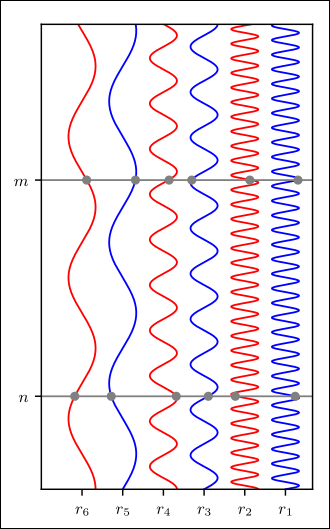
\includegraphics[width=0.6\textwidth]{_files/_images/positional_encoding}
\end{figure}
